\section{Understanding the Performance}
\label{sec:understand-perf}
In this section, we aim to have a better understanding of the end-to-end speedups reported in \autoref{sect:e2e-perf}. 
We start by breaking down where time and memory are spent on different SD stages -- drafting, verification, rejection sampling, and others, and how these keep us from reaching the theoretical upper bound. We then examine how acceptance patterns within a request, across requests, and across datasets. 

% While the $n$-gram approach, as a training-free SD variant, typically underperforms compared with learned SD methods in \autoref{sect:e2e-perf}, its acceptance patterns indicate untapped potential; in particular, we observe surprisingly long acceptance segments under specific conditions. This motivates a case study to investigate when this lightweight, training-free method can be especially advantageous.
% , linking prompt–output overlap, measured by BLEU-$n$ score~\cite{papineni2002bleu}, to the strong speedups achieved by the $n$-gram method. 

\subsection{End to End Speedup Formula}
As pointed in the original SD paper~\cite{leviathan2023fast},
Let $c$ denote the execution-time ratio of a single forward pass between the drafting method and the target model, $\alpha$ is the token acceptance rate and $k$ is the proposed length. The expected overall wall-time speedup achieved by speculative decoding, can be expressed as follows:\footnote{This formulation assumes that the $k + 1$ simultaneous evaluations of the target model take approximately the same amount of time as generating a single token in parallel. This assumption typically holds when the system is memory-bound, which is common at small batch sizes, but may break down once the system becomes compute-bound.}
\begin{equation}
\label{eq:speedup}
     E(speedup)=\frac{1-\alpha^{k+1}}{(1-\alpha)(kc+1)}.
\end{equation}
As shown, the speedup depends on two factors: the proposed length ($k$), the execution-time ratio between the drafting method and the target model ($c$), and the token acceptance rate ($\alpha$). Importantly, the absolute execution time of the drafting method is irrelevant; only its runtime relative to the target model affects the achievable speedup.

Employing a more sophisticated drafting method can improve the token acceptance rate $\alpha$, but often at the cost of increased execution time, leading to a larger $c$. Consequently, optimal speedup is achieved by carefully choosing a drafting method that balances the trade-off between $c$ and $\alpha$. In the following sections, we evaluate these factors and additionally analyze the memory overhead of SD.

\section{Execution Time and Memory Breakdown}
\label{sec:breakdown}
% \jerry{
% 1. describe figures
% 2. does percentage vary across model sizes (different TPs)?
% 3. verification cost is the majority
% }
% \lily{
% Old comments, migrated:
% 1. explain the speedup difference between measured ones in vLLM and eagle repo.
% 2. what's optimal speedup if we get rid of engineering overhead. explain we already cudagraph the propose/verify model, it's efficient.
% 3. add results of 70B model, add communication time.
% 4. discuss the potential of async scheduling.}

% \jerry{Should we explain why we didn't analyse time breakdown for draft-model based and MTP?}
\subsection{Execution Time}
% \lily{(1)We should include a detailed execution-time breakdown for draft-model–based methods in Section4.} 
In \autoref{fig:exec-breakdown}, we present the execution time breakdown of different stages in the baseline LLM execution and SD settings. For all experiments, we sample 500 requests from CNN/DailyMail. All other runtime settings are the same as \autoref{tab:exp-config}. 
For each configuration, we report the fraction of total execution time attributable to four components:
\textit{(i)}~\textbf{Drafting}, the time to generate speculated tokens, which corresponds to the lookup operation for $n$-gram and the autoregressive generation of the EAGLE heads for EAGLE and EAGLE-3;
\textit{(ii)}~\textbf{Verification}, the time spent by the target model to validate proposed tokens;
\textit{(iii)}~\textbf{Rejection Sampling}, time spent on generating final tokens based on verification logits;
and \textit{(iv)}~\textbf{Other Overheads}, all other overheads in the vLLM execution system. 

\begin{figure*}
\centering
\begin{subfigure}[t]{0.43\linewidth}

\includegraphics[width=\linewidth]{figures/time_breakdown/legend_only.pdf}
\end{subfigure}

\begin{subfigure}[t]{0.33\linewidth}
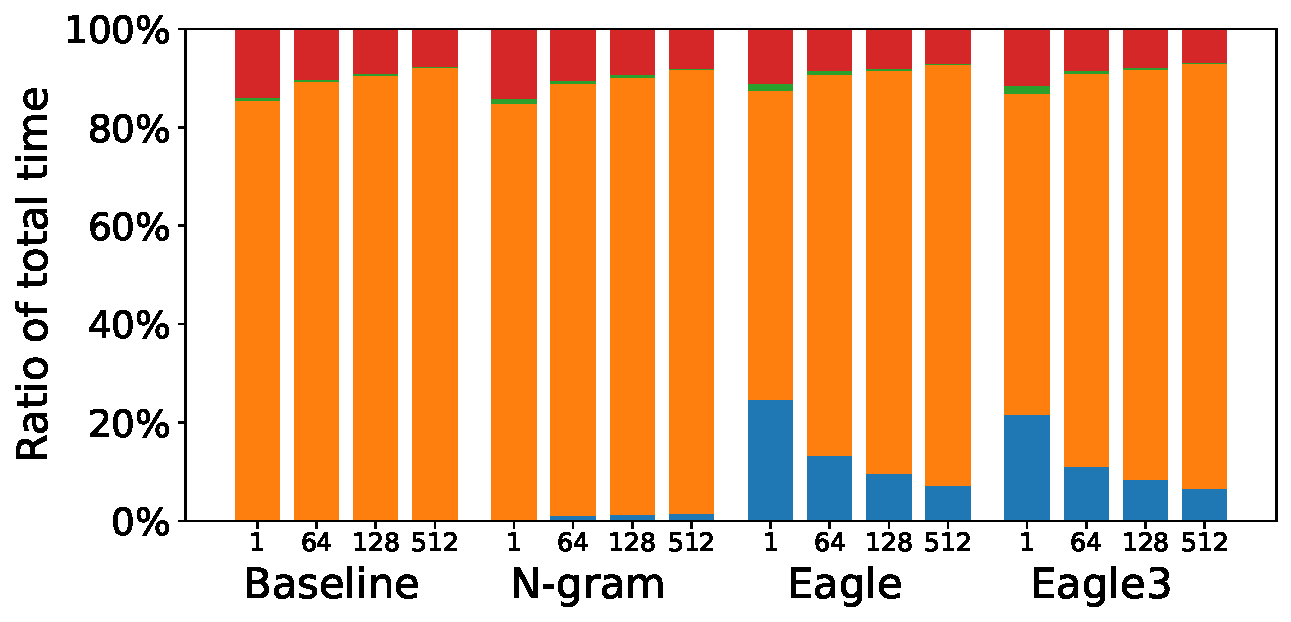
\includegraphics[width=\linewidth]{figures/time_breakdown/cnndailymail_llama3.1-8B_time_breakdown_legend_False.pdf}
\caption{Llama3.1-8B}
\end{subfigure}
\begin{subfigure}[t]{0.33\linewidth}
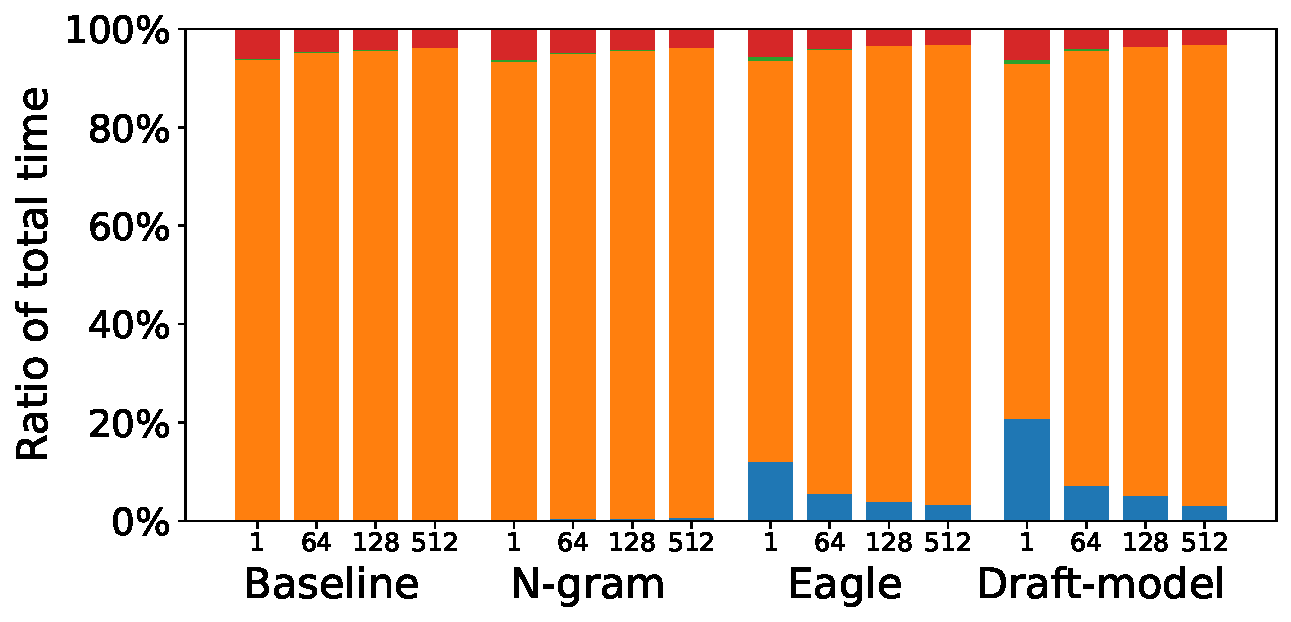
\includegraphics[width=\linewidth]{figures/time_breakdown/cnndailymail_Llama-3-70B_time_breakdown_legend_False.pdf}
\caption{Llama3-70B}
\end{subfigure}
\begin{subfigure}[t]{0.33\linewidth}
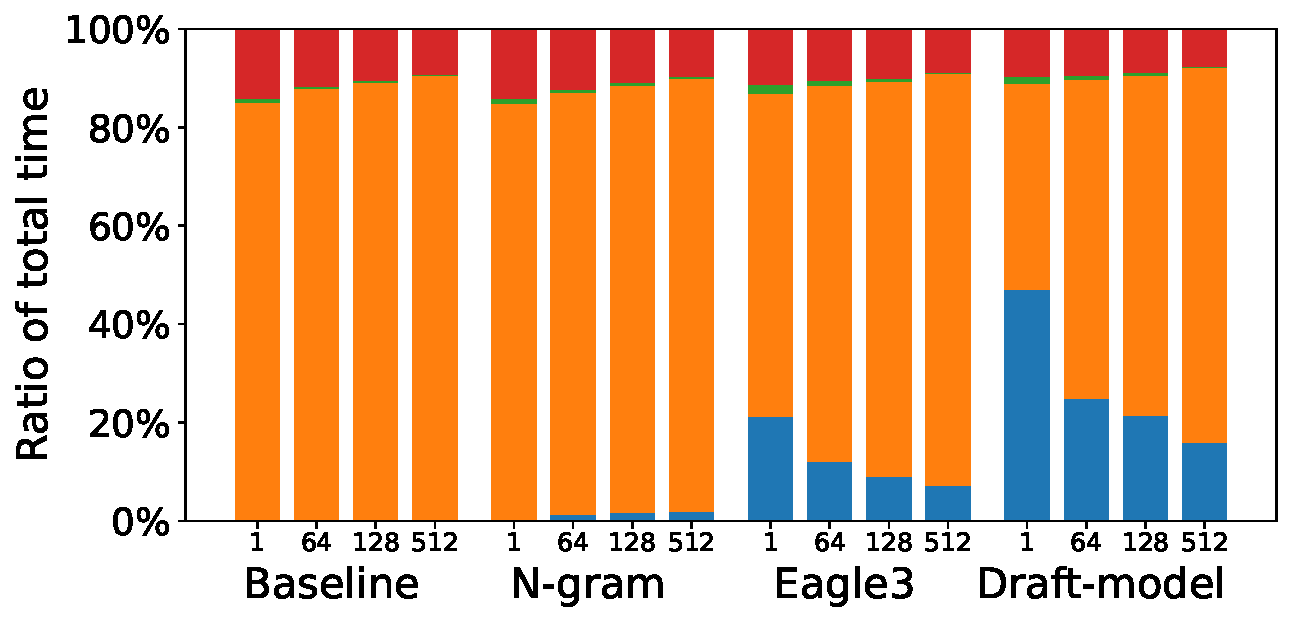
\includegraphics[width=\linewidth]{figures/time_breakdown/cnndailymail_Qwen-3B_time_breakdown_legend_False.pdf}
\caption{Qwen3-8B}
\end{subfigure}
\caption{Execution time breakdown across different models.}
\label{fig:exec-breakdown}
\vspace{-0.1in}
\end{figure*}


\begin{quoting}[leftmargin=1.5em, rightmargin=1.5em, vskip=0pt]
\textbf{Execution Time.}
% \emph{Verification time dominates across all speculative decoding variants, while sampling time is negligible. Drafting time is negligible for the $n$-gram method and remains below 20\% for EAGLE.}
\emph{Verification time generally accounts for the largest share of runtime across speculative decoding variants, while sampling time is negligible. Drafting is negligible for $n$-gram, stays below 20\% for EAGLE/EAGLE3, and stays under 40\% for draft-model methods acorss all batch sizes.}
\end{quoting}

We observe that the verification stage generally takes the largest execution time, ranging from 42\% to 95\% in all execution methods, which increases with the model size and batch size. 

Drafting costs, however, vary substantially by proposal mechanism. For $n$-gram, drafting time accounts for less than 2\% across all executions, adding negligible overhead to the baseline execution. Both EAGLE and EAGLE3 show similar drafting overhead characteristics, accounting for a 12\% to 20\% of the execution time at batch size 1, and 3\% to 7\% at batch size of 512.
Draft-model-based methods differ in that they must run a separate smaller model autoregressively to propose tokens, leading to a larger drafting overhead when the batch size is small. For Llama3-70B, drafting takes from 21\% at batch size of 1 to 3\% at batch size of 512. For Qwen3-8B, drafting is about 47\% at batch size of 1 and decreases to 16\% at batch size of 512. As a result, the verification fraction is correspondingly lower (roughly 72\% for Llama3-70B and 42\% for Qwen3-8B at batch size of 1). 
% Verification still remains the dominant component in general, except for Qwen3-8B at batch size of 1, where drafting is slightly larger.

% For drafting, $n$-gram drafting time accounts for less than 2\% across all executions, adding negligible overhead to the baseline execution. Both EAGLE and EAGLE3 show similar drafting overhead characteristics, accounting for a 12\% to 20\% of the execution time at batch size 1, and 3\% to 7\% at batch size of 512.
% As such, even if EAGLE-based speculative decoding may provide a better acceptance rate, it may be beneficial to use $n$-gram over EAGLE when the model or the batch size is small, as shown in more detail later.
Furthermore, the sampling stage takes a negligible amount of time, accounting for less than 1.7\% of total time across all executions. 
% While the vLLM's system overhead increases slightly with the batch size, the increase is marginal compared to the increase in the verification time. 
Lastly, vLLM overhead accounts for 3–12\% of total execution time. This fraction decreases as model and batch size grow, since fixed overheads—such as scheduling—are independent of model scale and therefore become amortized at larger batch size or model size.

\textbf{Implication.} Verification cost dominates the end-to-end execution of speculative decoding, indicating that running the large target model remains the primary computational bottleneck. When the proposed tokens are ultimately accepted, this cost is well justified. However, verifying tokens that are later rejected can incur substantial wasted computation. This observation motivates a natural question: how much of the verification compute is truly useful? Conversely, what speedup could be achieved if verification were performed only on “correct” tokens, eliminating wasted work? These questions form the basis of \autoref{sec:theoretical-speedup}, where we estimate the theoretical upper bound for SD.

\subsection{Memory}
In \autoref{tab:memory}, we present the GPU memory usage of each SD variant with Llama3.1-8B, Llama3-70B and Qwen3-8B.
% , excluding the vLLM system overhead, such as memory fragmentation in KV cache blocks. 
We use FP-16 precision and report the static memory overhead from the model weights and per-token KV cache calculated using model specs. We do not report intermediate memory overheads, such as the activation tensors during execution. The detailed calculation steps can be found in \autoref{appendix:mem}.

\begin{table}[t] % Use [htbp] for better float placement
    \small
    % --- First Sub-table ---
    \begin{subtable}[t]{\columnwidth}
        \centering
        \begin{tabular}{c|c|c|c}
             \toprule
              & No SD/$n$-gram & EAGLE & EAGLE 3\\
             \midrule        
             Static (GiB) & 14.96 & 15.43 & 15.75 \\
             Per-token (KiB) & 128 & 132 & 132 \\
             \bottomrule
        \end{tabular}
        \caption{Memory breakdown on Llama3.1-8B} % Optional caption for sub-table (a)
        \label{tab:sub1} % Label for the first sub-table
    \end{subtable}
    \hfill % This command pushes the two subtables apart
    % --- Second Sub-table ---
    \begin{subtable}[t]{\columnwidth}
        \centering
        \begin{tabular}{c|c|c|c}
              \toprule
              & No SD/$n$-gram & EAGLE & D-M (1B)\\
             \midrule        
             Static (GiB) & 131.4 & 133.3 & 133.7 \\
             Per-token (KiB) & 320 & 324 & 352\\
             \bottomrule
        \end{tabular}
        \caption{Memory breakdown on Llama3-70B} 
        \label{tab:sub2} % Label for the second sub-table
    \end{subtable}
    \hfill
    \begin{subtable}[t]{\columnwidth}
        \centering
        \begin{tabular}{c|c|c|c}
              \toprule
              & No SD/$n$-gram & EAGLE3 & D-M (0.6B)\\
             \midrule        
             Static (GiB) & 15.25 & 16.00 & 16.37 \\ 
             Per-token (KiB) & 144 & 148 & 256\\
             \bottomrule
        \end{tabular}
        \caption{Memory breakdown on Qwen3-8B} 
        \label{tab:sub3}
    \end{subtable}
    
    \caption{Static and per-token memory usage of the baseline model execution and different speculative decoding methods. DM stands for Draft-Model-based method.}
    \label{tab:memory} % The main label for the combined table
    \vspace{-0.1in}
\end{table}


\begin{quoting}[leftmargin=1.5em, rightmargin=1.5em, vskip=0pt]
\textbf{Memory.}
\emph{Speculative decoding generally incurs minimal memory overhead, including both static parameters and KV cache: it is zero for $n$-gram, below 10\% for EAGLE/EAGLE-3, while draft-model-based methods incur overhead that depends on the chosen draft model.}
\end{quoting}
% We also do not report memory overhead required for $n$-gram token lookup, as it is done entirely on the CPU.
We find that the memory overhead of speculative decoding (SD) is minimal. For $n$-gram SD, draft tokens are sampled from CPU-resident generation history, incurring no GPU memory overhead. 

\textbf{Static Memory.} Static memory corresponds to the memory required to store model weights. Certain SD variants add extra layers or even an independent model, thereby incurring additional static memory overhead. EAGLE-based SD introduces an additional Transformer layer and thus requires extra static weights, but the overhead is small: 3.1\% (EAGLE)/ 5.3\% (EAGLE3) for Llama-3.1-8B, 1.4\% (EAGLE) for Llama-3-70B, and 4.9\% (EAGLE3) for Qwen3-8B.
For draft-model-based SD, static memory overhead depends on the size of the draft model; in our setup, pairing Llama-3-70B with Llama-3.2-1B incurs a 1.8\% increase while pairing Qwen3-8B with Qwen3-0.6B incurs a more significant 7.3\% increase. 

\textbf{Per-token Memory.} Per-token memory refers to the size of the KV cache allocated for each generated token. The total KV cache footprint grows with the number of generated but unfinished requests. Consequently, for workloads with long generation lengths such as reasoning workloads, memory cost introduced by KV cache becomes a dominant factor in overall memory consumption.
Per-token overhead is modest for EAGLE-based methods, as each EAGLE layer requires the same KV cache as a single attention layer (4 KiB per token), resulting in a 3.1\% overhead for Llama-3.1-8B and 1.3\% for Llama-3-70B. 
In contrast, draft-model–based SD incurs substantially higher per-token memory overhead, as it relies on an additional multi-layer model for token proposal. In our configuration, pairing a 0.6B draft model with an 8B target model increases the per-token memory footprint from 144 KiB to 256 KiB, corresponding to a 1.77$\times$ increase.



% \textbf{Observation.} \lily{TODO, small bach size, enough memory.}



% \begin{figure*}[h]
%     \centering
%     \includegraphics[width=0.24\linewidth]{figures/time_breakdown/cnndailymail_llama3.1-8b_none_128_time_ratios.pdf}
%     \includegraphics[width=0.24\linewidth]{figures/time_breakdown/cnndailymail_llama3.1-8b_ngram_128_time_ratios.pdf}
%     \includegraphics[width=0.24\linewidth]{figures/time_breakdown/cnndailymail_llama3.1-8b_eagle_128_time_ratios.pdf}
%     \includegraphics[width=0.24\linewidth]{figures/time_breakdown/cnndailymail_llama3.1-8b_eagle3_128_time_ratios.pdf}
%     \caption{Histogram of execution time breakdown for Llama3.1-8B (TP=1) model.}
    
%     \includegraphics[width=0.3\linewidth]{figures/time_breakdown/cnndailymail_Qwen_Qwen3-8B_none_128_time_ratios.pdf}
%     \includegraphics[width=0.3\linewidth]{figures/time_breakdown/cnndailymail_Qwen_Qwen3-8B_ngram_128_time_ratios.pdf}
%     \includegraphics[width=0.3\linewidth]{figures/time_breakdown/cnndailymail_Qwen_Qwen3-8B_eagle_128_time_ratios.pdf}
%     \caption{Histogram of execution time breakdown for Qwen3-8B (TP=1) model.}

%     \includegraphics[width=0.3\linewidth]{figures/time_breakdown/cnndailymail_meta-llama_Meta-Llama-3-70B-Instruct_none_128_time_ratios.pdf}
%     \includegraphics[width=0.3\linewidth]{figures/time_breakdown/cnndailymail_meta-llama_Meta-Llama-3-70B-Instruct_ngram_128_time_ratios.pdf}
%     \includegraphics[width=0.3\linewidth]{figures/time_breakdown/cnndailymail_meta-llama_Meta-Llama-3-70B-Instruct_eagle_128_time_ratios.pdf}
%     \caption{Histogram of execution time breakdown for Llama3-70B (TP=4) model.Time ratio: time spent on the given phase divided by the total execution time of the step. \jerry{change histogram to a bar chart!}}

%     \label{fig:exec-breakdown}
% \end{figure*}
